\documentclass{beamer}

\usepackage{paratype}
\setbeamerfont{frametitle}{family=\bf}
\usepackage{listings}

\lstset{
  language=C,
  keepspaces=true,
  moredelim=**[is][\color{red}]{@}{@},
}

% Beamer theme settings
\usecolortheme{seagull}
\usenavigationsymbolstemplate{} % no navigation buttons

\usepackage[utf8]{inputenc}

\title{OpenCL day 1: GPU hardware and the programming model}

\author{Cosmin Oancea and Troels Henriksen}

\date{January 28, 2019}

\begin{document}

\frame{\titlepage}

\section{Introduction and Course Contents}

\begin{frame}
  \tableofcontents[currentsection]
\end{frame}

\section{Hardware Trends}

\begin{frame}
	\tableofcontents[currentsection]
\end{frame}

\begin{frame}
  \frametitle{A graph of CPU progress}

  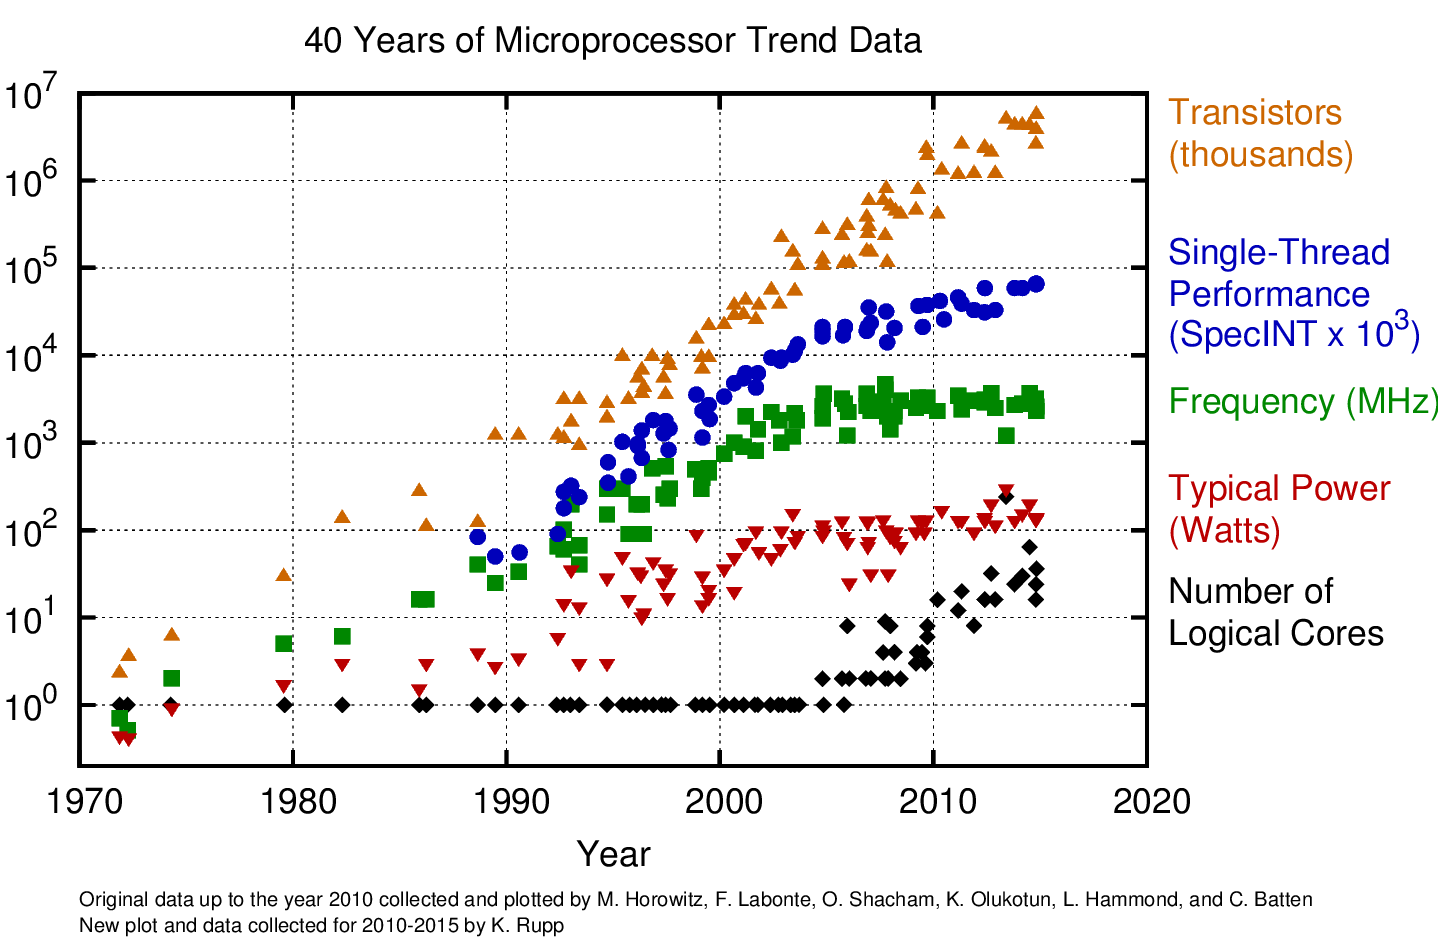
\includegraphics[width=\textwidth]{img/40-years-processor-trend.png}

\end{frame}

\section{CPU vs GPU architectures}

\begin{frame}
	\tableofcontents[currentsection]
\end{frame}

\begin{frame}
  \frametitle{GPUs vs CPUs}

  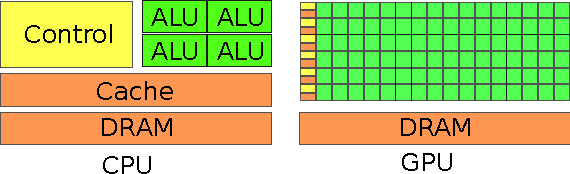
\includegraphics[width=\textwidth]{img/cpu-gpu-architecture.pdf}

  \begin{itemize}
  \item GPUs have \textit{thousands} of simple cores and taking full
    advantage of their compute power requires \textit{tens of
      thousands} of threads.
  \item GPU threads are very \textit{restricted} in what they can do:
    no stack, no allocation, limited control flow, etc.
  \item Potential \textit{very high performance} and \textit{lower
      power usage} compared to CPUs, but programming them is
    \textit{hard}.
  \end{itemize}

  \textbf{Massively parallel processing is currently a special case,
    but will be the common case in the future.}
\end{frame}

\section{The OpenCL programming model}

\begin{frame}
	\tableofcontents[currentsection]
\end{frame}

\section{Debugging and Profiling OpenCL}

\begin{frame}
	\tableofcontents[currentsection]
\end{frame}

\begin{frame}[fragile,fragile]
  \frametitle{Profiling with Wall Clock Time}

Just like how you profile anything else.

\begin{lstlisting}
// Current wall time in microseconds.
static int64_t get_wall_time(void);
\end{lstlisting}

Use it like this:

\begin{lstlisting}
int64_t before = get_wall_time();

...

clFinish(ctx);

int64_t after = get_wall_time();

printf("Took %d microseconds\n",
       (int)(after-before));
\end{lstlisting}

The \lstinline{clFinish()} call is crucial as otherwise the device may
still be working (remember that most enqueuings are
\textit{asynchronous}).

\end{frame}

\begin{frame}[fragile]
  \frametitle{Profiling with Events}

  An event is an object that communicates the status of an OpenCL
  command.  Whenever we enqueue something in a command queue, we can
  get an event object back.

\begin{lstlisting}
 cl_int clEnqueueNDRangeKernel
   (cl_command_queue command_queue,
    cl_kernel kernel,
    cl_uint work_dim,
    const size_t *global_work_offset,
    const size_t *global_work_size,
    const size_t *local_work_size,
    cl_uint num_events_in_wait_list,
    const cl_event *event_wait_list,
    @cl_event *event@)
\end{lstlisting}

\end{frame}

\begin{frame}[fragile]
  \frametitle{Retrieving Information from Events}

\begin{lstlisting}
cl_int clGetEventInfo
  (cl_event event,
   cl_event_info param_name,
   size_t param_value_size,
   void *param_value,
   size_t *param_value_size_ret)
\end{lstlisting}

\begin{lstlisting}
 cl_int clGetEventProfilingInfo
   (cl_event event,
    cl_profiling_info param_name,
    size_t param_value_size,
    void *param_value,
    size_t *param_value_size_ret)
\end{lstlisting}

  The latter only works if \lstinline{CL_QUEUE_PROFILING_ENABLE} was
  passed to \lstinline{clCreateCommandQueue()}.
\end{frame}

\begin{frame}[fragile]
  \frametitle{Values for \texttt{cl\_profiling\_info}}

  \begin{description}
  \item[\texttt{CL\_PROFILING\_COMMAND\_QUEUED}]\hfill\\ When the
    command was queued.
  \item[\texttt{CL\_PROFILING\_COMMAND\_SUBMIT}]\hfill\\ When the
    command was sent to the device.
  \item[\texttt{CL\_PROFILING\_COMMAND\_START}]\hfill\\ When the
    command started executing.
  \item[\texttt{CL\_PROFILING\_COMMAND\_END}]\hfill\\ When the
    command finished executing.
  \end{description}

  \begin{itemize}
  \item All produce a value of type \lstinline{cl_ulong}.
  \item \lstinline{clGetEventProfilingInfo()} returns
    \lstinline{CL_PROFILING_INFO_NOT_AVAILABLE} if the information is
    not available (yet)
  \end{itemize}
\end{frame}

\begin{frame}[fragile]
  \frametitle{Example of Profiling with Events}

\begin{lstlisting}
cl_event write_e;
clEnqueueWriteBuffer(queue, to, CL_FALSE,
                     0, n,
                     from,
                     0, NULL, &write_e));

...

cl_ulong start, end;

clGetEventProfilingInfo
  (write_e, CL_PROFILING_COMMAND_START,
   sizeof(start), &start, NULL);
clGetEventProfilingInfo
  (write_e, CL_PROFILING_COMMAND_START,
   sizeof(end), &end, NULL);
\end{lstlisting}

\end{frame}

\begin{frame}
  \frametitle{Event Profiling versus Wall Clock Profiling}

  \begin{itemize}
  \item Event profiling is \textbf{much more fine-grained} and lets us
    see the per-operation runtime.
  \item Measuring per-operation with wall clock would require us to
    \texttt{clFinish()} after every operation, which is very slow
    because it prevents pipelining.
  \item Wall clock profiling tells us about \textbf{overall
      application performance}.  We generally cannot just sum the
    runtimes for each event, since the commands may overlap in time,
    and the events do not count host-based overheads.
  \item \textbf{Ideally, use both.}
  \end{itemize}

  However, neither of these approaches will tell us \textit{why}
  something is slow...
\end{frame}

\section{Programming Exercises}

\begin{frame}
	\tableofcontents[currentsection]
\end{frame}


\end{document}

%%% Local Variables:
%%% mode: latex
%%% TeX-master: t
%%% End:
